\section{Problem Model and Motivating Example} \label{sec3}
\noindent
To explain our problem, we consider a control application system consisting of an ensemble of concurrently active control applications / loops. Each control application is partitioned into a set of
tasks. The control tasks communicate via a shared bus. The messages on the shared bus are also scheduled using a given arbitration policy. When a control loop executes, it carries out the set of tasks as specified by different states in its control state machine. Among all these states, some
states require bus access, for which the control loop presents a request to the bus arbiter. These requests are considered by the bus arbiter / scheduler which decides on a bus scheduling strategy to grant bus access to the different control loops over time at different time slots. \\

\noindent
As discussed in recent literature, we consider each participating control application is modeled as a B\"{u}chi automaton. B\"{u}chi automatons~\cite{leeuwen90/Thomas90} have been a popular mechanism of choice for modeling applications that require finite automatons over infinite strings or words. The basic structure of such automatons is similar to their finite counterparts, with the exception of the acceptance conditions, as described below.
A B\"{u}chi automaton is described as a five tuple, 
$A = (Q,I,\delta,q_0,F)$, where $Q$ is a finite set of states, $I$ is the input alphabet, $\delta : Q$ x $I \rightarrow Q $ is the transition function, $q_0$ 
is an initial state ($q_0 \in Q$) and $F$ is a set of final states that help us model the infinitary acceptance condition. An infinite word $\lambda \in I ^ \omega$ over the input alphabet takes the automaton through an infinite sequence of states $ q_0, q_1, q_2, ....$, which describes a run of
the automaton such that $ q_{k+1} \in \delta(q_k, \delta_k)$ where $k \in \mathbb{N}$ and $\delta_k$ refers to the $k^{th}$ symbol on the input 
word $\delta$. An infinite word is accepted if some 
accepting state $q_f \in F $ appears in the run $ q_0, q_1, q_2, ....$ 
infinitely often. If 
$|\delta(q,i)| = 1$ where $ q \in Q $ and $i \in I$, then it is a deterministic 
B\"{u}chi automaton, otherwise it is non-deterministic. \\

\noindent
Each control loop is designed with a control objective in view, and the overall functioning of the system is dependent on the individual control loops meeting control objectives, along with a strategy for co-operative control of the shared message bus through which the control loops communicate with each other. We consider one such control system functioning correctly if both the above conditions are met. Meeting control objectives has been addressed in several recent articles, and is therefore, not discussed here. In contrast, we focus more on the schedulability aspect, as described below. 

\subsection{Schedulability and code replacement attack:} 
\noindent
We now characterize the schedulability requirement below. 
A set of concurrent control loops, each expressed as a B\"{u}chi automaton, is considered {\em schedulable} if there exists a strategy to schedule the individual control loops on the shared bus {\em infinitely often}.
The scheduling objective is defined in the lines of infinitary acceptance, as is the case with B\"{u}chi objectives. Intuitively, a scheduler should be able to allocate bus access to each individual control loop infinitely often. More specifically, given any infinite run of the composed system, at least one constituent task (i.e. bus accessing / accepting state) from each control loop should repeat infinitely often. We consider the system {\em safe} if this holds, {\em attacked} otherwise. We conclude that a {\em code replacement attack} has been carried out if a system,  initially safe and schedulable, turns out to be non-schedulable. 

\begin{figure}
\begin{center}
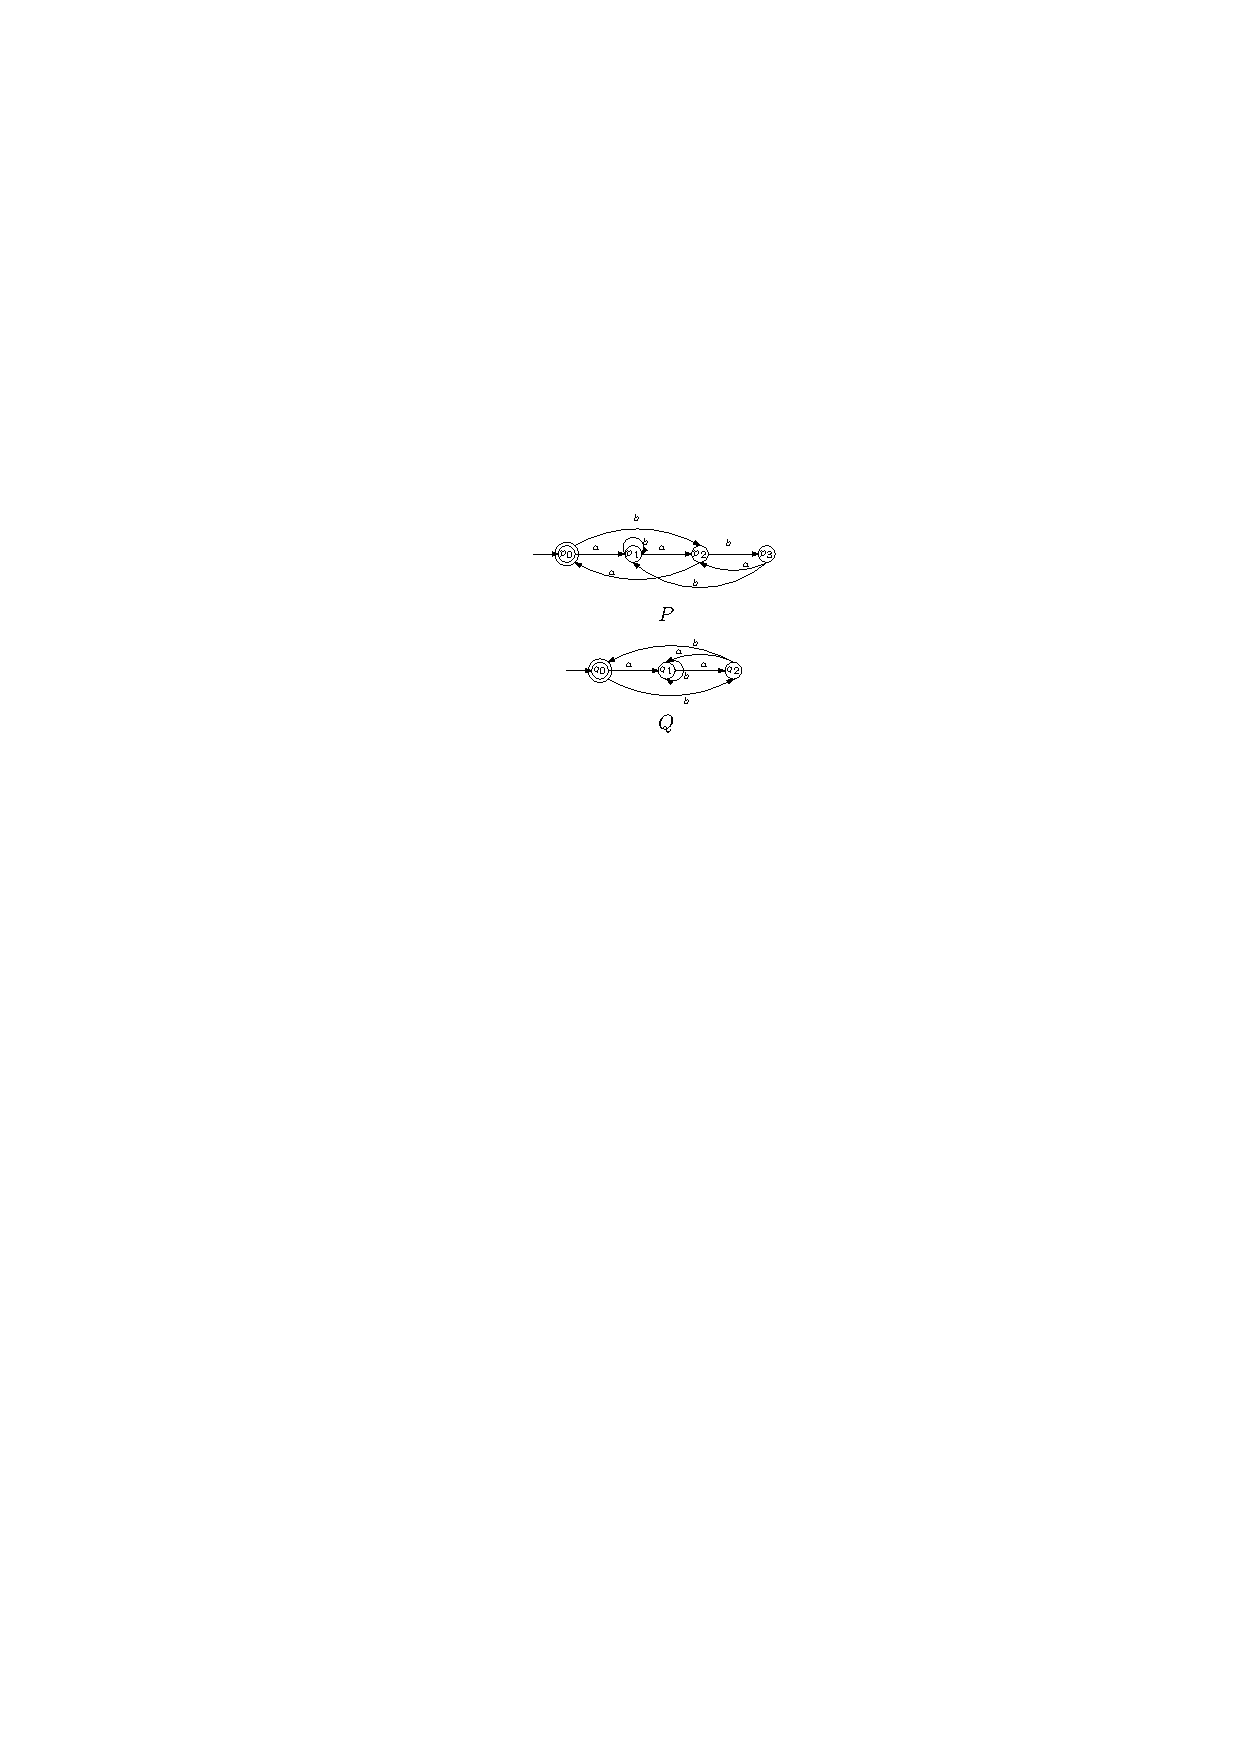
\includegraphics[width=50mm]{motivating_example_automata.pdf}
\end{center}
%\vspace{-0.1in}
\caption{{\em Initial Control loops}}
\label{state}
\end{figure}

\subsection{Motivating Example:}
\noindent
We explain our problem statement with a small example. Fig\ref{state} presents two automatons $P$ and $Q$  representing two different control applications.
Each has one initial state and an acceptance state. The acceptance states are the bus accessing states
of the automaton. The  schedulability of the system is depicted using timing diagram in Fig \ref{state-transition}

In the diagram, time is plotted along the horizontal axis and the schedulers are plotted along the vertical axis. The timing diagram depicts how the control
applications are scheduled with the bus scheduler. The scheduler gives access to the slot to $P$ control application at every $5th$ occurance. Other slots 
are accessed by $Q$ control application. 


\noindent
We now consider, a code replacement attack takes place on this system. The resulting automaton is depicted in Fig \ref{replaced}.
As a result of this attack, one of the control loops $P$ is changed, as a result of which, there is a change in the structure of the scheduling sequence of the bus scheduler. 
After the replacement the $P$ control application is unable to access the bus.  As we can see in Fig \ref{state-transition},
there are no access from $P$ control application which satisfy our infinitary scheduling condition,
thus schedulability is no longer guaranteed and we conclude that a code replacement attack has taken place.

\begin{figure}
\begin{center}
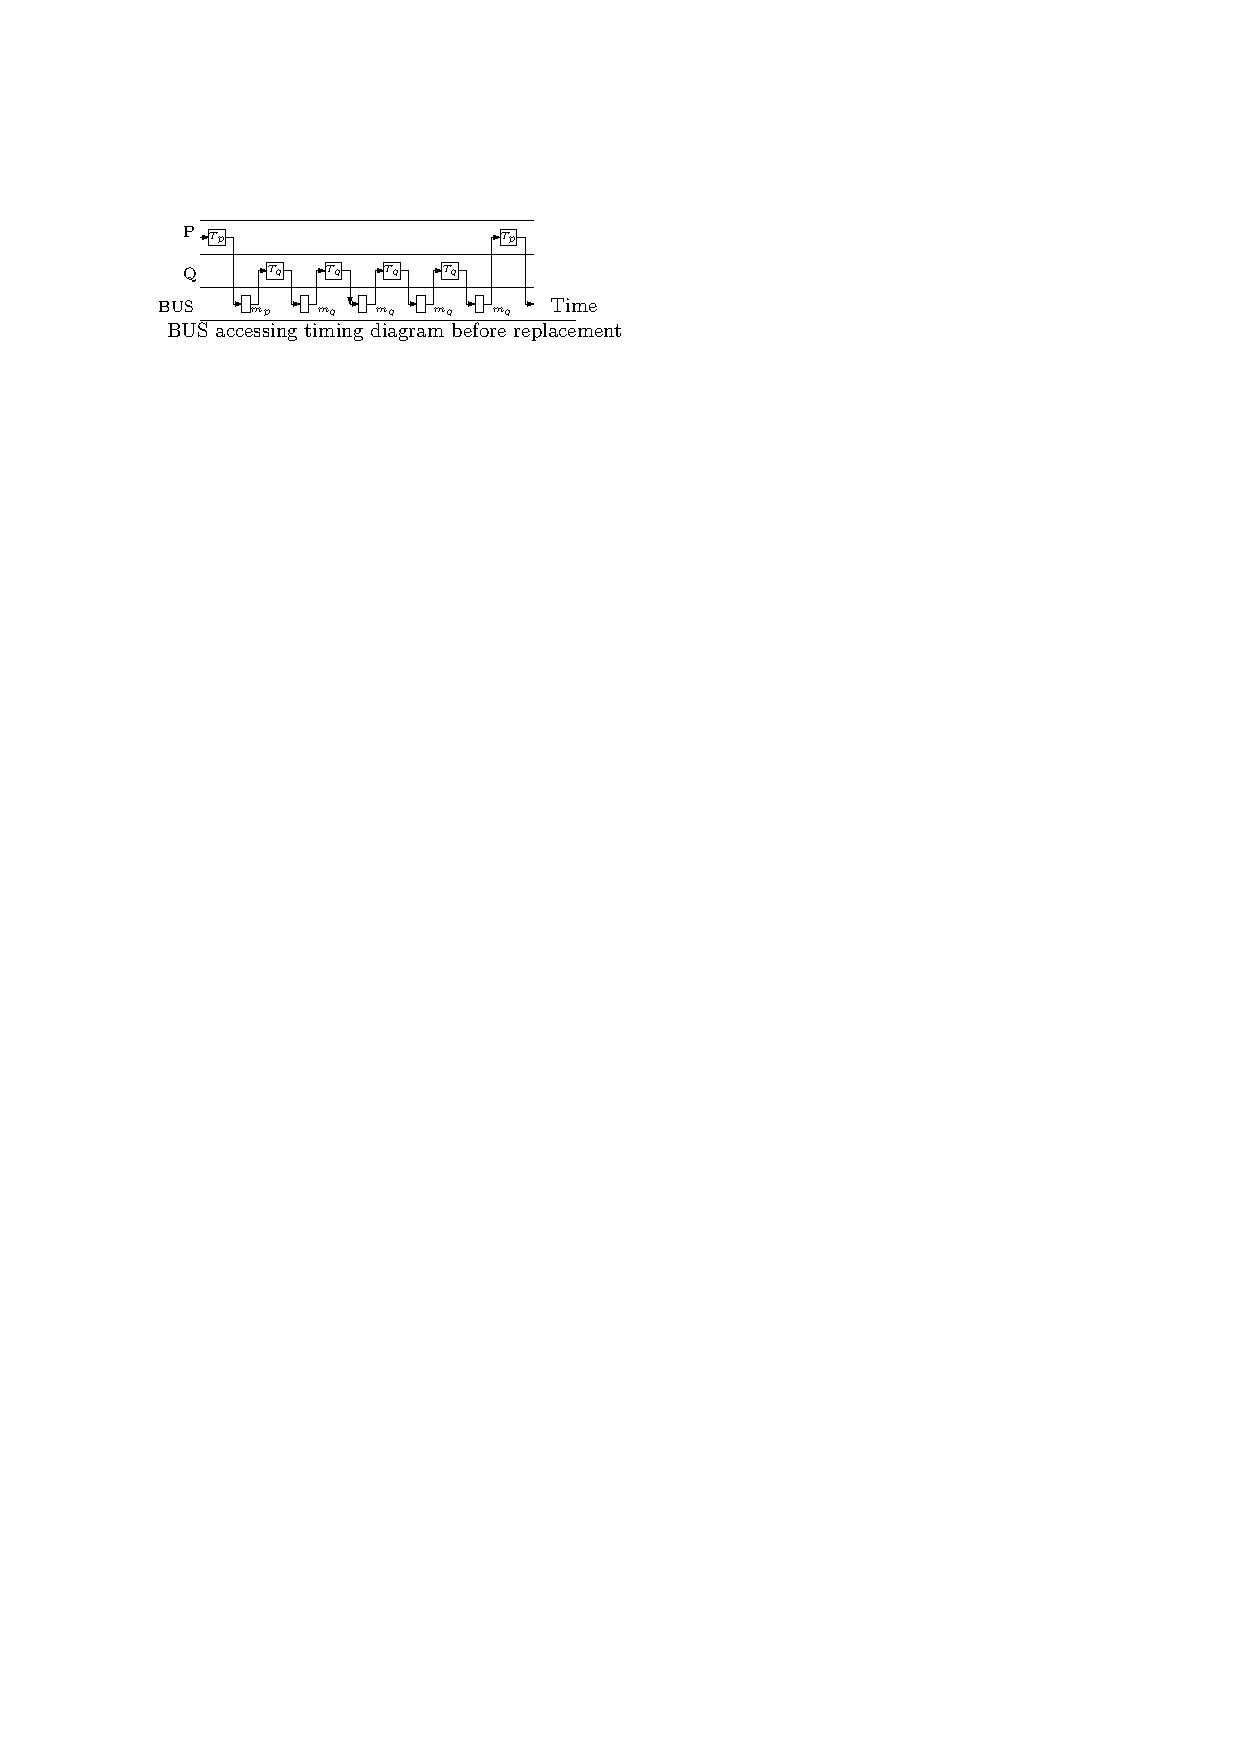
\includegraphics[width= 75mm]{bus_timing_diagram.pdf}
\end{center}
%\vspace{-0.1in}
\caption{{\em Timing diagram of bus scheduler, before and after replacement}}
\label{state-transition}
\end{figure}

\begin{figure}
\begin{center}
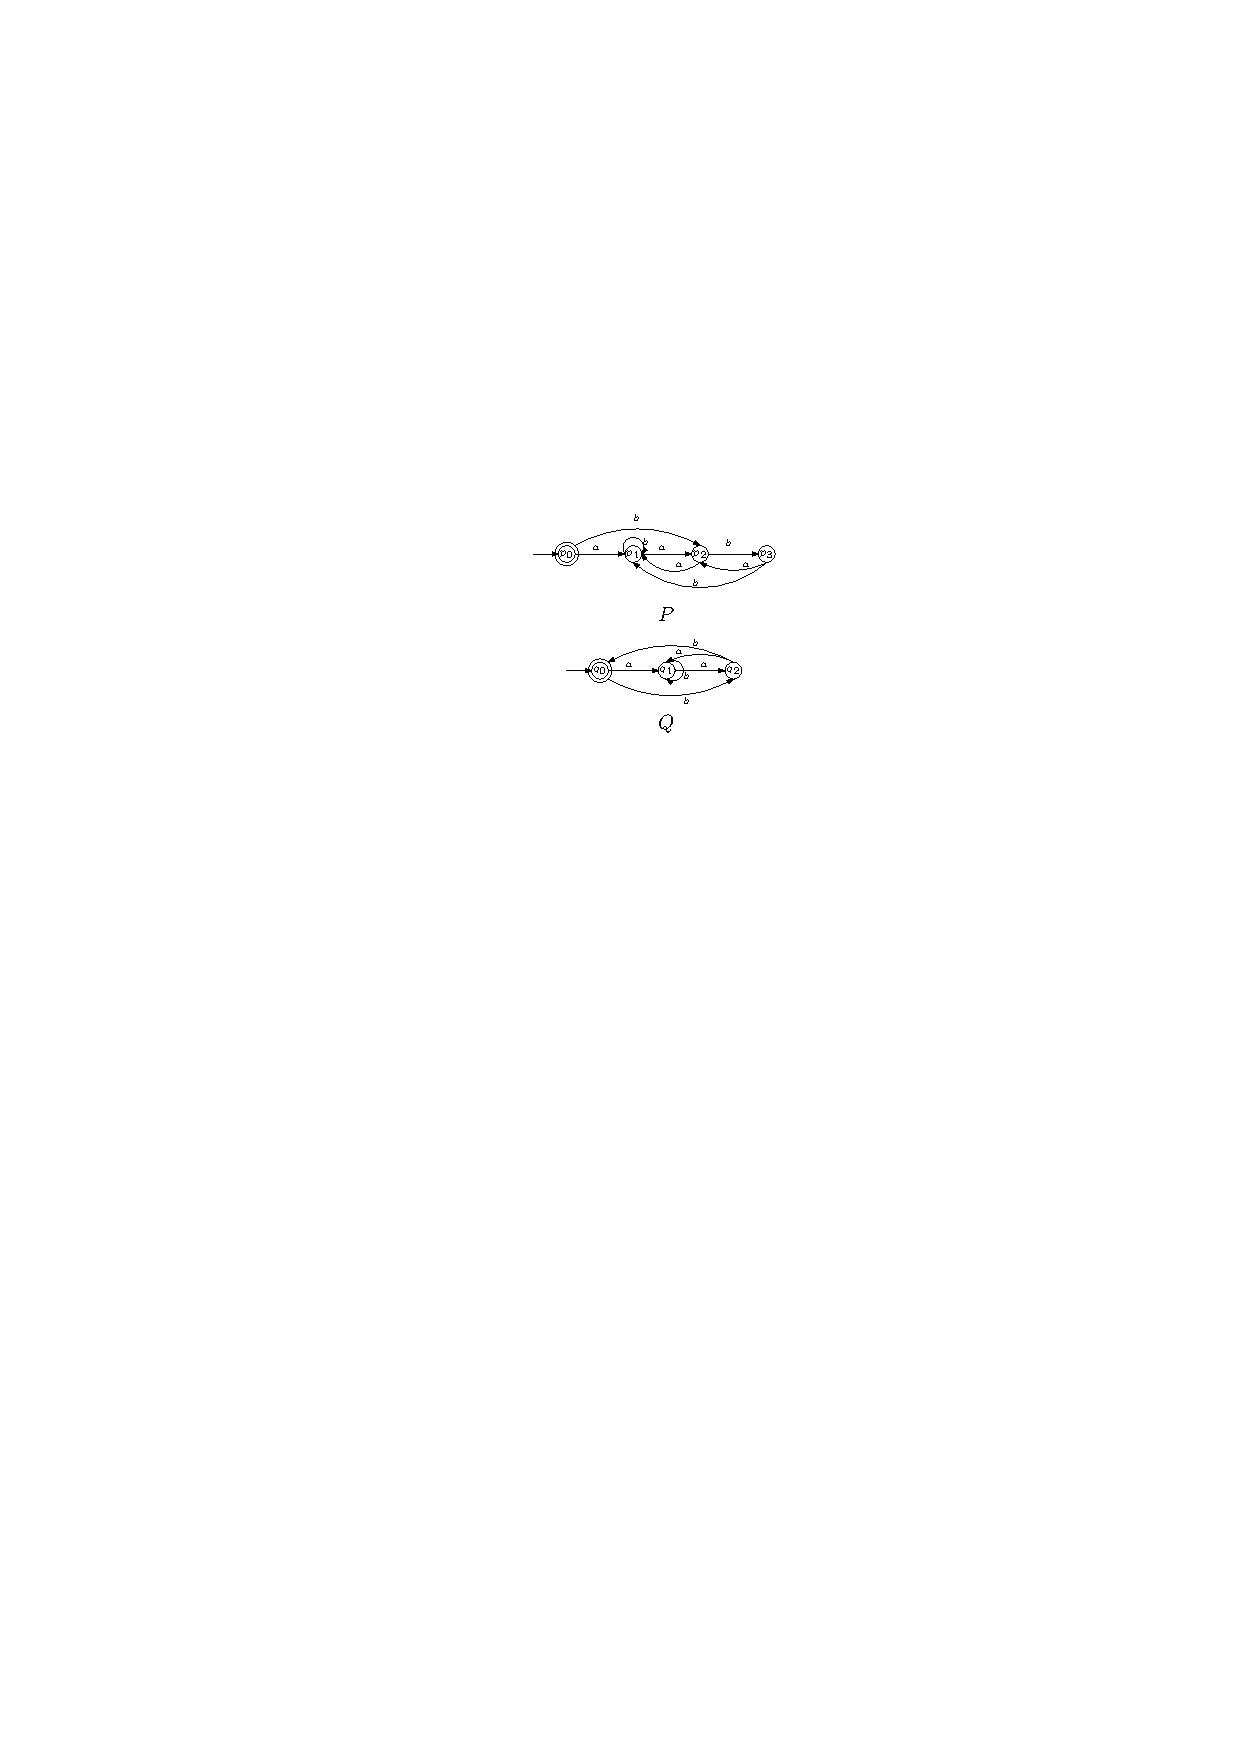
\includegraphics[width= 50mm]{motivational_example_replaced.pdf}
\end{center}
%\vspace{-0.1in}
\caption{{\em Modified control loops after a replacement attack}}
\label{replaced}
\end{figure}



